\section{Deep neural networks in tracking}
Trackers based on deep learning have been researched because of \ac{dnn}s' ability
to capture hierarchies of features from raw data with minimal earlier domain specific
knowledge. They provide greater versatility compared to traditional trackers that are
based on hand-crafted sets of features. This chapter reviews both early research
done in the field and more recent trackers that have made use of \ac{dnn}s.

\subsection{Early works}
Multilayered \ac{cnn}s are currently common as feature extractors, but an implementation
of a \ac{cnn}-based tracker~\cite{HUMAN_CNN} pre-dates the work of Krizhevsky et.
al.~\cite{NIPS_IMAGENET} that sparked the current research on \ac{dnn}s for classification
tasks. Fan et.~al.~\cite{HUMAN_CNN} proposed a shift-variant architecture utilizing the
previous tracking result each frame. They recognized crowded scenes containing multiple
objects similar to the target to be especially challenging as false positives could result
in drift from the intended target. A reference position from the previous frame was used
to provide additional information for locating the target in the current one. They also
considered the shift-invariance of conventional detection \ac{cnn}s to present its
own challenges. Shift-invariance means that the position of an object does not affect the
network's output, which is beneficial for classification tasks as it is desirable to
recognize the objects in an image regardless of their position. However, a tracker is
expected to identify the location of the target, which motivated the adoption of a
shift-variant architecture.~\cite{HUMAN_CNN}

\begin{figure}[H]
\centering
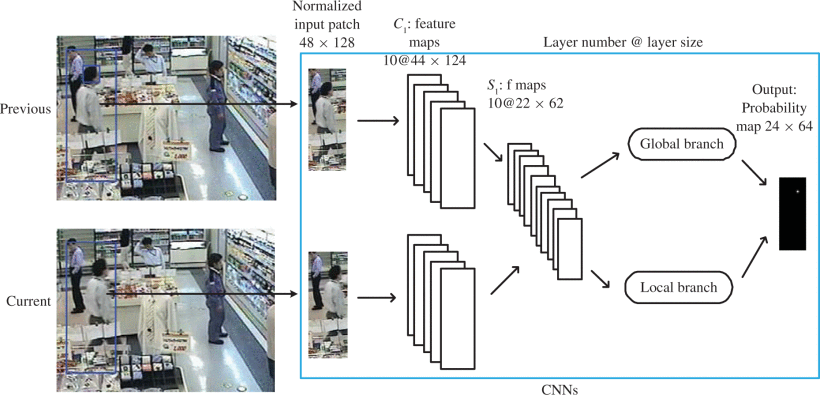
\includegraphics[width=1\textwidth]{human_cnn}
\caption{The network Fan et.~al.~\cite{HUMAN_CNN} featured a branching desing to
         include two consecutive frames in the extracted features as well as to detect
         structures of features on both a local and global scale. Source: Fan et.
         al.~\cite{HUMAN_CNN}}\label{fig:human_cnn}
\end{figure}

The tracker Fan et.~al.~presented had separate input layers for extracting feature
maps from the current and previous frame (fig.~\ref{fig:human_cnn})~\cite{HUMAN_CNN}.
These were then downsampled together before splitting the rest of the convolutions
into two branches to obtain both global and local structures of features. Global
structures were extracted with a series of convolutions, while local structures were
discovered by sampling the branching output with a single convolution. The network's
final layer took the outputs of both branches and produced the final probability map
based on them.~\cite{HUMAN_CNN}

Training of the network was performed on a set of 20,000 images obtained from
surveillance videos and it was supervised by comparing the probability map resulting from
a pair of frames to a target map. Online tracking was done on a fixed model to avoid the
drift adaptive models can induce. The proposed tracker performed especially well when the
arget's position or the view changed as the tracker was trained to track humans
specifically. Even so, only being able to track a single class of targets is a major
limitation.~\cite{HUMAN_CNN}

Another influential tracker, the \ac{dlt}~\cite{DLT}, was a general object tracker
consisting of a pre-trained \ac{sdae} and an additional classification layer. Their goal
was to combine philosophies of generative and discriminative trackers by developing a
discriminative tracker that learns and uses an effective image representation. The
\ac{sdae} was trained to extract generic image features using 1 million randomly sampled
images from the Tiny Images dataset~\cite{TINY_IMAGES} of 80 million images labelled by
their main subject. After training, a sigmoid classification layer was added to the
encoder part of the \ac{sdae} to complete the tracker. The model could also be tuned
during tracking if a significant change in the target's appearance is detected. Tracking
could achieve an average frame rate of 15 frames/s on a GPU, which is sufficient for many
real-time applications. The tracker also compared favorably to then state of the art
trackers on a set of 10 video sequences.~\cite{DLT}

\subsection{Current state of the art}
These trackers include some of the novel approaches that have been researched in the
recent years.

\subsubsection{Evolution of Deep Learning Tracker}
The ideas behind \ac{dlt} were developed further by Wang et.~al.~\cite{LEARNED_HIERARCH}.
They observed that \ac{dlt} couldn't obtain deep features with temporal invariance due to
training on unrelated images instead of videos. Another remark was that \ac{dlt} doesn't
have an integrated objective function to adapt the encoder to a target as the weights are
only updated if the target appearance seems to have changed during tracking. The new
\ac{cnn} based feature learning method was integrated into an existing tracking system
called ASLSA~\cite{ASLSA}, which originally used raw pixel values as its
representations.~\cite{LEARNED_HIERARCH}

The two layer feature model learned features capable of handling complicated motion
transformations based on the work of Zou et.~al.~\cite{INVARIANT_FEATS}. It was trained
on auxiliary video sequences and the goal was to learn features invariant between two
frames, which results high-level features strong against non-linear motion patterns. These
generic features didn't include appearance information of specific target objects so a
domain adaptation module was added to both layers to readjust them according to a
specific target.~\cite{LEARNED_HIERARCH}

Evaluation on some challenging sequences showed that the tracker Wang et.~al.~\cite{LEARNED_HIERARCH}
proposed could track targets that underwent non-rigid object deformation and in- or
out-of-plane rotations. It was also observed to perform better than the baseline trackers
and beat \ac{dlt} in 5 of the 8 sequences tested. However, the tracker was implemented
as a single-threaded CPU program and it only reached 0.6 frames/s in comparison to the 15
frames/s of the GPU implementation of \ac{dlt}~\cite{DLT}.

\subsubsection{Tracking of severely blurred objects}
The work of Ding et.~al.~\cite{BLUR_TRACK} focused on the issue of motion blur. They noted
that generic trackers assume to have a blur free video to work with, while motion blur is
very common in real videos. It was stated that the performance of such trackers may drop
significantly if applied to videos with severe motion blur and two challenges were
noted in such situations: the appearance features of the object are damaged by blur
and abrupt motion of it is difficult to estimate. Deblurring the input was dismissed as
too computationally costly and potentially prone to change appearance features.~\cite{BLUR_TRACK}

A \ac{sdae} trained on blurred images was proposed as a solution for capturing blur-invariant
features. The layers were first pre-trained in sequence and in an unsupervised setting,
but fine-tuning of the model was done on all layers simultaneously. Only the encoding
layers were used after the joint training.~\cite{BLUR_TRACK}

When initializing the online tracker, the positive samples retrieved by sampling around
the target are blurred using kernels simulating combinations of different magnitudes
and directions of blur to produce a model less affected by blur effects. Not blurring
the training samples might result in tracking failure or drift if abrupt and severe
motion blur occurs in the beginning of the sequence. The background is sampled around
the initial bounding box for negative samples and those are used without transformations.
Tracking results are stored during tracking to update the model if a significant
appearance change is detected by the maximum confidence dropping below a set
threshold.~\cite{BLUR_TRACK}

Evaluation was done in two parts. First, severely blurred videos were used to test
performance with severe blur and abrupt motion. After that, commonly used challenging
sequences were used to evaluate general performance in difficult conditions. The new
tracker performed well in both scenarios as it placed in the top two trackers in several
categories and good results were shown overall. Real-time tracking seems also feasible
as the tracker ran at 5--10 frames/s on a quad-core CPU and moderately powerful GPU while
the implementation was said to have room for optimization.~\cite{BLUR_TRACK}

\subsubsection{DeepTrack}
DeepTrack~\cite{DEEPTRACK} is a \ac{cnn} based tracker capable of competitive performance
with training occurring entirely during tracking. They attributed the difficulties of
adopting \ac{cnn}s in tracking to a limited amount of positive training samples available
in the tracking sequences, a tendency to overfit to the most recent observation and pure
computational intensity. Their method employed a special type of loss function that
consisted of a structural term and a truncated norm. The structural term was included
to positive samples with different significance levels depending on the uncertainty of
the object location and the truncated norm helped to reduce the number of samples needed
in back-propagation to accelerate training.~\cite{DEEPTRACK}

The network consisted of two convolutional layers and two fully connected layers (fig.~\ref{fig:deeptrack}).
It was trained on multiple low-level features extracted from the image such as normalized
gray-scale image and image gradient. Each cue had its own branch of layers. These
layers were trained before substituting the fully connected layers of all channels
with a common fusion layer for joint training. The fusion layer was responsible for
final labeling in the tracking process.~\cite{DEEPTRACK}

\begin{figure}[H]
\centering
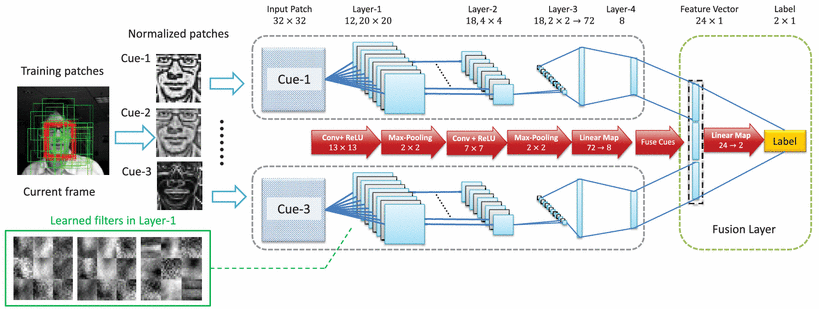
\includegraphics[width=1\textwidth]{deeptrack}
\caption{DeepTrack extacted three cues from each frame and each of them were passed
         to their own branch of two convolutional layers and two fully connected ones.
         A fusion layer then combined their outputs to the final output.~\cite{DEEPTRACK} Source: Li et.
         al.~\cite{DEEPTRACK}}\label{fig:deeptrack}
\end{figure}

The model was only updated when a significant change appearance change was detected
and the fusion layer was updated using a slower rate than the preceding feature layers.
The feature representations were assumed to change fast and each image cue to contribute
more stably. Update was also constrained by having the window of positive samples in
memory be longer than that of negative samples. This was done to reduce overfitting.
The positive samples past the first frame were also judged less than reliable and
were assigned a label noise value that was taken into account when the model was updated.
DeepTrack was shown to outperform other trackers in two benchmarking challenges
spanning 60 video sequences and it reached framerates of 2--4 frames/s on powerful
hardware.~\cite{DEEPTRACK} While not exactly real-time for all applications, the
framerates are comparable to other methods.

\subsubsection{Multi-Domain Network}
Another novel tracker, Multi-Domain Network~\cite{MDNET}, used domain specific
classification layers (fig.~\ref{fig:mdnet}). Each video was treated as a separate domain
and had their own branch after the generic layers. The generic layers consisted of three
convolutions and two fully connected layers, while the branching domain specific
classifiers were all a single fully connected layer for solving the binary classification
problem between the target and its background. Training was done iteratively by training
on a single domain per iteration but alternating between domains. Through this process,
domain independent information was modelled to obtain generic feature representations
that were resilient to common variations such as illumination changes and scale
variations.~\cite{MDNET}

\begin{figure}[H]
\centering
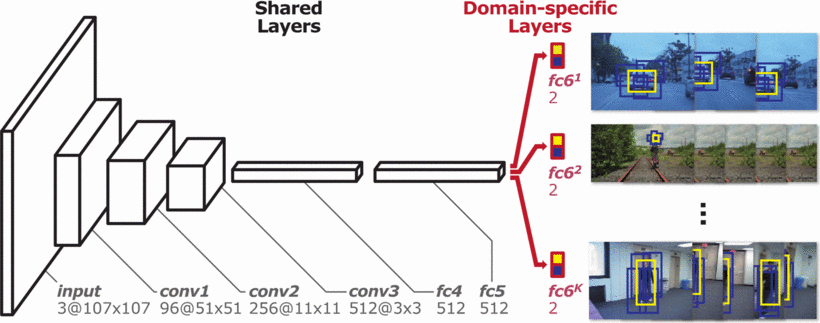
\includegraphics[width=0.8\textwidth]{mdnet}
\caption{A depiction of the Multi-Domain Network. This form was used during training
         to train generic features with a domain specific final classification layer.
         The online version replaced the branches with a single randomized classifier
         to be tuned during tracking.~\cite{MDNET} Source: Nam and Han~\cite{MDNET}}\label{fig:mdnet}
\end{figure}

In online tracking, the domain specific branches are substituted by a single randomly
initialized layer that is tuned during tracking along with the shared fully connected
layers. Model updates were handled by separate mechanisms for long and short term updates.
Short term updates were only done if tracking failure was detected, while long term updates
were performed at regular intervals using positive samples gathered over a long period.
Both methods used negative samples from a short period since old negative samples are
redundant or irrelevant to the current frame. Evaluation of the tracker showed good
performance in two benchmarks with other tracking algorithms. A tracking speed of
1 frame/s was reached on a quad-core CPU and moderately powerful GPU.~\cite{MDNET}

\subsubsection{Fully convolutional tracker}
Wang et.~al.~\cite{FCN_TRACK_2} observed that many of the earlier works treated \ac{dnn}s
as black-box classifiers. They took a different approach and studied the properties of
\ac{cnn} features from the perspective of online visual tracking. Two realizations
emerged from the results. First, different properties from different depths of features
fit the problem. High-level features help distinguishing object classes while lower
layers provide features for discerning the target from distracters. The new tracker
(fig.~\ref{fig:fcn}) was designed to switch between the two types based on the current
distracters. Second, the features trained on classification data are for distinguishing
generic objects and some of them might serve as noise in tracking. Thus, a method was
proposed for discarding noisy or unrelated feature maps for the target.~\cite{FCN_TRACK_2}

\begin{figure}[H]
\centering
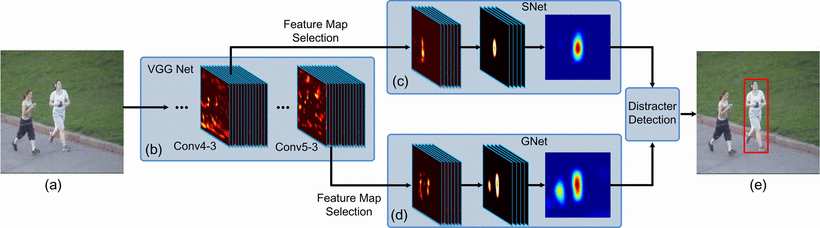
\includegraphics[width=1\textwidth]{fcn_track}
\caption{Two branches of convolutions evaluated the target position from different
         levels of features and the branch used in determining the position was decided
         based on the current scene. Source: Wang et.~al.~\cite{FCN_TRACK_2}}\label{fig:fcn}
\end{figure}

The tracker was built on top of the 16-layer VGG network~\cite{VGG} and the layers
conv4\textunderscore3 (10th) and conv5\textunderscore3 (13th) were chosen as the two
levels of features used. Conv4\textunderscore3 was connected to a ``specific network''
that discriminated the target from the background and Conv5\textunderscore3 fed a
``general network'' that captured category information. The VGG network had been
pre-trained but the branches were initialized on the first frame of the tracking
sequence. The two branches both output a heatmap and a distracter detection scheme
determined which was to be used. After the first frame, updates were only done to
the specific network using a setup similar to that of the Multi-Domain Network~\cite{MDNET}.
Framerates of 3 frames/s were reached on a powerful GPU with competitive performance in
a benchmark.~\cite{FCN_TRACK_2}

\authorcomment{
%\cite{DISCR_SALIENCY}
Combines a pre-trained feature descriptor \ac{cnn} and a SVM that creates a
saliency map from the extracted features. This map is used as a filter to extract
the position of the target in each frame.

%\cite{SIAM_TRACK}
Applies a siamese architecture of two convolutional networks to object tracking.
A candidate image is compared to an exempla image and is scored based on their
similarities.

%\cite{SPAT_RCN}
Combines an efficient feature extractor (YOLO) to spatial and temporal constraints.
The network's layers are first pre-trained with a traditional \ac{cnn} for general
feature learning. YOLO is then adopted as the detection module and the \ac{lstm}
is added before training it as part of the whole network. The \ac{lstm} is provide
robust access to long-range context and is fed with the output of the detection
stage converted to a 32x32 heatmap linked with the learned visual features.

%\cite{HIERARCH_FEATS}
Instead of using just the final output of a sequence of convolutional layers, the
proposed algorithm uses multiple layers to find the target's position. This is done
by going through the outputs coarse-to-fine to regularize the search for the maximum
value in the finer response maps. All the layers' correlation filter numerator and
denominator are also updated each frame to get a robust and computationally lighter
approximation of minimizing output error.

%\cite{FCN_TRACK}
Views the traditionally fully connected layers at the end of a \ac{cnn} based
tracking network as convolutional layers and uses upscaling with skip connections
to previous layers. This \ac{fcn} is computationally lighter than a sliding window
based network as it only requires a single feedforward [connection?]. The network
was pre-trained on the VOC2012 dataset to learn features for targets of 20 categories
in the dataset. The tracker is only able to detect objects in those categories.
It also only allows single object tracking but the target can be identified in the
first probability map if the sequence contains multiple targets to permit multi-object
scenarios and increase accuracy in single-object tracking. (However, the method is
currently not efficient enough for tracking in real time.)

%\cite{SMS_DLT}
Uses a \ac{sdae} fine-tuned with SURF features gotten from matching the current frame's
to the first one's.
}